\section{Summary and Future works}
\subsection{Summary}
In this chapter, we discussed the importance of defect control and the challenges that the standard approach faces in implementing it. We then derived $4^{th}$, $6^{th}$ and $8^{th}$ order Hermite-Birkhoff interpolants (HB4, HB6, HB8) that were used to augment the Classical $4^{th}$ order Runge-Kutta method (RK4). We showed that HB4 is not an appropriate way to provide an interpolant for defect control of RK4 as the interpolation error of the derivative is of a lower order than the numerical solution computed by RK4. We then showed that HB6 provides reliable and efficient defect control and that HB8 does not provide much of an improvement over HB6. We next showed how the HB6 and HB8 interpolants can be used to augment $6^{th}$ and $8^{th}$ order Runge-Kutta methods to allow them to provide efficient defect control. We also noted throughout the chapter that the multistep interpolants HB6 and HB8 have accuracies that rely on their step-size parameters, $\alpha$ and $\beta$, being close to 1. We then discussed an interpolant that forces these parameters to be 1 by using the evaluations of previous interpolants.

paragraph on asympt and error control.

\subsection{Future Works}
\label{section:HB_future_work}

\paragraph{The first few steps}
Throughout this chapter we have used the exact solution values for the first few steps in order to allow us to create the first interpolant. Another important research project in this area is to try different techniques including but not limited to the use of CRK methods, error control with a sharper tolerance than the user provided tolerance, and possibly other methods to perform the first few steps.

\paragraph{Asymptotically correct defect control with multistep interpolants}
paragraph on HB6 that we developed and potential for HB8.

We can also look into developing interpolants that could lead to asymptotically  correct defect control. 
This would guarantee that the maximum defect is always at the same relative location within each step and would thus only require one function evaluation to sample the defect.

\paragraph{HB10}
An idea for future work is to derive a $10^{th}$ order interpolant. Such an interpolant will be forced to use 3 step-size parameters but an idea is to fix one or more of the parameters at 1. This can be done by using the technique that we employed in Section $\ref{section:keeping_alpha_at_1}$ or by using another technique such as computing a solution value in the middle of the step $[x_{i-1}, x_i]$ using the interpolant from that step and performing an additional function evaluation at that data point to obtain the two values required to build an interpolant. Thus we get to use just two parameters $\alpha$ and $\beta$ for the step from $x_i$ to $x_{i+1}$ and the step from $x_{i-2}$ to $x_{i-1}$.  This will give the required 10 data points to produce such an interpolant which could then be used to augment RK8 to provide a more efficient defect control scheme for the $8^{th}$ order case. 

Early explorations into creating an HB10 interpolants seem to be promising. See Figure $\ref{fig:future_work_hb10_v_shape}$ to see how an HB10 derived by `breaking the middle step' is resilient to changes to its parameters $\alpha$ and $\beta$. We note that the interpolant was built with step-size $[\alpha h, \frac{h}{2}, \frac{h}{2}, \beta h]$ and thus $\alpha$ and $\beta$ is usually 2 when there are no step-size changes. We also note that $\theta$ was allowed to vary between $-2-\alpha$ to $\beta$.

\begin{figure}[H]
\centering
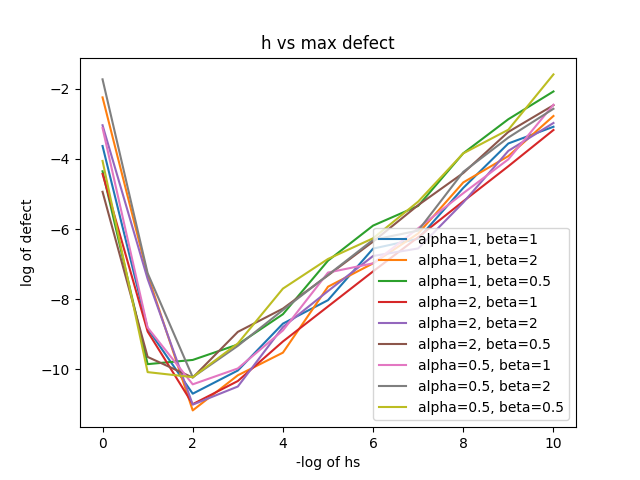
\includegraphics[width=0.7\linewidth]{./figures/future_work_hb10_v_shape}
\caption{V-shape of HB10 created by `breaking the middle step'.}
\label{fig:future_work_hb10_v_shape}
\end{figure}
